\documentclass{article}
\usepackage[utf8]{inputenc}
\usepackage{hyperref}
\usepackage{graphicx}
\graphicspath{ {./images/} }

\title{Agile Software Projects}
\author{}
\date{November 2020}

\begin{document}

\maketitle
\tableofcontents
\listoffigures
\newpage

\section{Aims and Objectives}
\subsection{Product Goals \& Value Proposition}
\emph{Set clear goals and concise and appropriate challenges which are measurable. Aims should be specific, with your objectives building up a bigger picture of what you hope to do. Goals and operations should be clearly specified.}

\subsection{Usability Goals}
\textit{The theme of usability is key.}

\subsection{Measuring Success}
\textit{This section should set out the measuring criteria for your work and your presentation will be judged in relation to these aims and objectives.}

\section{Market Analysis}
Our project does not have a direct competitor. There are some utilities which partially solve the problem we are tackling - namely, tracking grades - but none of these enable the user to compare themselves to their peers, nor aggregates grade data. As such, we must cast a wide net to analyze our place in the market and consider the \textit{alternative solutions}. We have identified these utilities which overlap with our project as well as tools which solve analogous problems in different domains in order to get a more comprehensive picture of where our product stands in the market.
\subsection{Overview of Alternative Solutions}
Our solution offers two mains functions: tracking grades and sharing/comparing grades. For each feature, we have documented the alternative solutions and their specific functionality and notable design choices.
\subsubsection{Grade Tracking}
\begin{enumerate}
  \item Peer's Python command line grade calculator
  \item Peer's Google Sheets Degree Planner
  \item gpacalculator.io
  \item University of London Portal
\end{enumerate}

\noindent The peer-created utilities and University of London portal were discovered through our teammates' participation in this course. gpacalculator.io is an example of many similar utilities that were found by searching 'grade tracking' and 'grade calculator' in Google.
\medskip

\noindent \textbf{1. Peer's Python command line grade calculator}

\noindent \url{https://github.com/sglavoie/grades_calculator}
\bigskip

\noindent Users record their grades in a JSON file and run the script from the command line to see grade and other relevant information
\bigskip

\begin{figure}[h]
\noindent 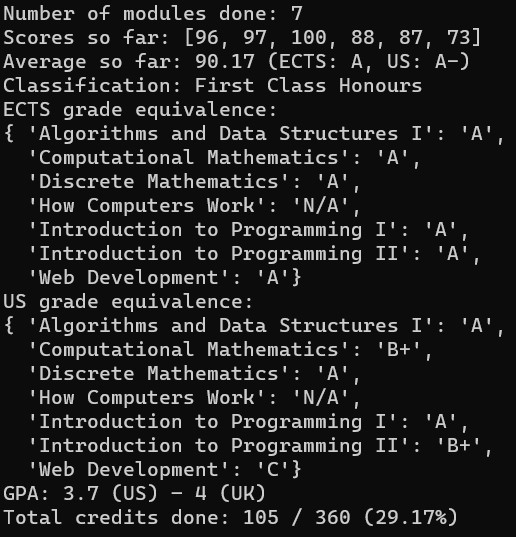
\includegraphics[height=200pt]{py-example-output}
\centering
\caption{Python calculator example output}
\label{fig: py-calc}
\end{figure}

\noindent \textbf{Features:}
\begin{itemize}
\item Track course and cumulative grades
\item Converts to ECTS (Europe) and US scale
\item Converts to US / UK GPA
\item Determines which classification your grades fall into
\item Tracks total credits done out of 360
\end{itemize}
\medskip

\noindent \textbf{Design Choices:}
\begin{itemize}
\item Command line utility with input coming from JSON
\end{itemize}
\medskip

\noindent \textbf{2. Peer's Google Sheets Degree Planner}

\noindent \sloppy \url{https://docs.google.com/spreadsheets/d/1w5mFDaEB86q9zj-sdn_FZ8ivu5ALSfPsvBw8iOZ7qkY/edit#gid=0}
\bigskip

\noindent Users records their grades in a Google sheet to track their credits and grades.
\bigskip

\begin{figure}[h]
\noindent 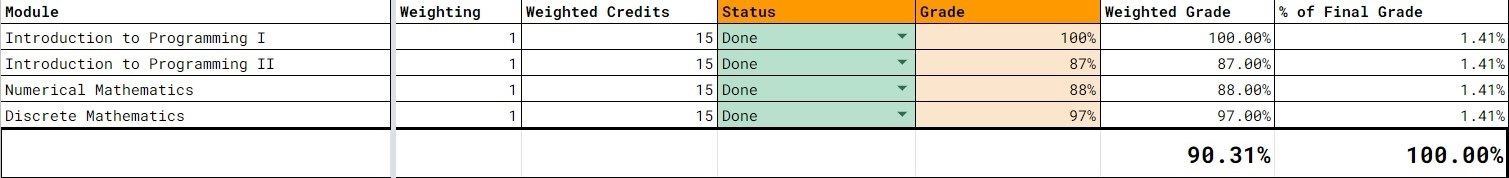
\includegraphics[width=\textwidth]{degree-planner-partial}
\centering
\caption{Example excerpt from Google Sheets Degree Planner}
\label{fig: deg-planner}
\end{figure}

\noindent \textbf{Features:}
\begin{itemize}
\item Track course and cumulative grades
\item Tracks total credits done out of 360
\item Shows which modules are optional
\end{itemize}
\medskip

\noindent \textbf{Design Choices:}
\begin{itemize}
\item implemented on google sheets
\item easy to share link
\end{itemize}
\medskip

\noindent \textbf{3. gpacalculator.io}

\noindent \url{https://gpacalculator.io}
\bigskip

\noindent Users enters there grades in web form and sees cumulative results.
\bigskip

\begin{figure}[h]
\noindent 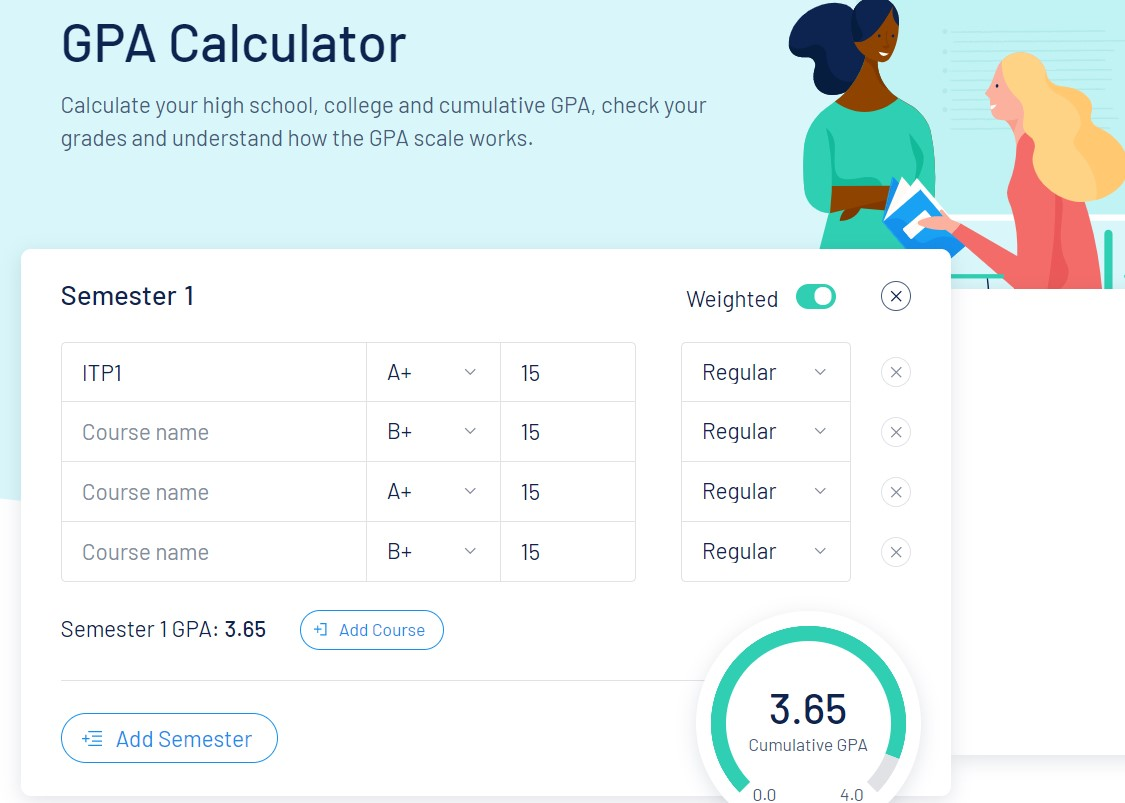
\includegraphics[height=200pt]{gpa-calculator-io}
\centering
\caption{Prominent landing page form on gpacalculator.io}
\label{fig: gpa-calc}
\end{figure}
\medskip

\noindent \textbf{Features:}
\begin{itemize}
\item Calculate semester or total cumulative GPA from individual courses
\item Offers different calculators for high school and college
\item General information about GPA, grades, and different honors
\end{itemize}
\medskip

\noindent \textbf{Design Choices:}
\begin{itemize}
\item Input form is prominently placed. Immediately confronted with it when visiting the page.
\item No login or form of persistence
\item US specific
\end{itemize}

\noindent \textbf{4. University of London Portal}

\noindent \url{https://my.london.ac.uk/group/student}
\bigskip

\noindent Users can view grades from each semester, broken down by source (coursework vs. exam).
\bigskip

\begin{figure}[h]
\noindent 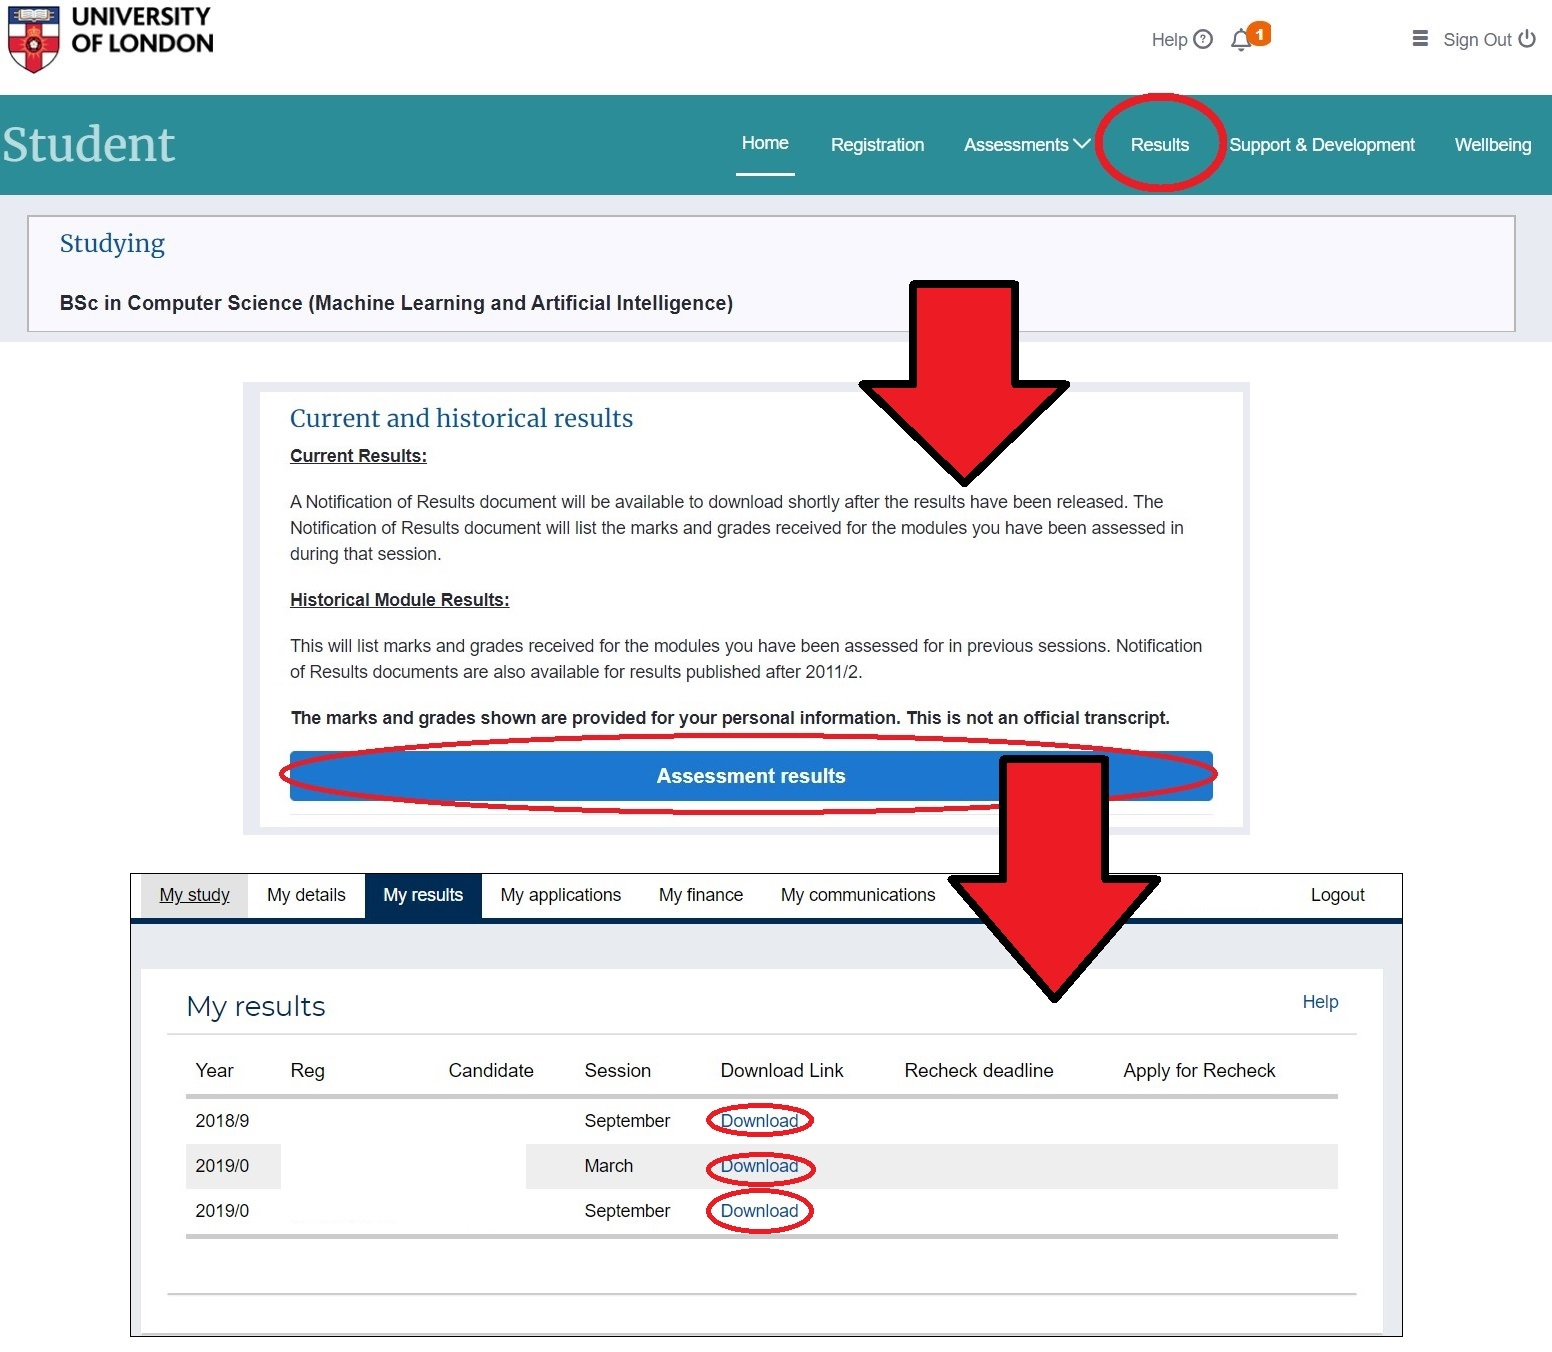
\includegraphics[height=250pt]{uol-buried}
\centering
\caption{Path to find grade download links on University portal}
\label{fig: uol-grades}
\end{figure}

\noindent \textbf{Features:}
\begin{itemize}
\item Shows grade results for each semester
\item Granular - shows grades for coursework and exam portion separately
\end{itemize}
\medskip

\noindent \textbf{Design Choices:}
\begin{itemize}
\item Buried deep in menus
\item No centralized place to view all grades nor cumulative grades
\item download required for all but most recent results
\end{itemize}
\medskip

\subsubsection{Grade Sharing}
\begin{enumerate}
  \item University of London Slack workspace
  \item glassdoor.com
\end{enumerate}

\noindent We searched Google for 'grade sharing,' 'grade comparing,' 'compare grades to other students,' and other derivatives but found no relevant tools. Glassdoor was suggested as an analogous tool during a brainstorming session and the slack workspace is known to us through our participation in the degree program.
\medskip

\noindent \textbf{1. University of London Slack workspace}

\noindent \sloppy \url{https://app.slack.com/client/TDT1N1BUG/C01A9AR0A4C}
\bigskip

\begin{figure}[h]
\noindent 
\includegraphics[height=200pt]{slack-share}
\centering
\caption{Students sharing midterm results and comparing to each other in course slack channel}
\label{fig: slack-share}
\end{figure}

\noindent This is the slack space open to all University of London online CS students. There are channels for each course. Grades are sometimes shared in threads after they are released.
\bigskip

\noindent \textbf{Features:}
\begin{itemize}
\item Impromptu sharing
\item Irregular
\item Not solicited
\end{itemize}
\medskip

\noindent \textbf{Design Choices:}
\begin{itemize}
\item Reports tend to be from people with high grades, or people with low grades who suspect an error with their results
\end{itemize}
\medskip

\noindent \textbf{2. glassdoor.com}

\noindent \url{https://glassdoor.com}
\bigskip

\noindent A review and reporting website for employers. Collects textual reviews and salary data from users. Salary reports are analogous to grade reports.
\bigskip

\begin{figure}[h]
\noindent 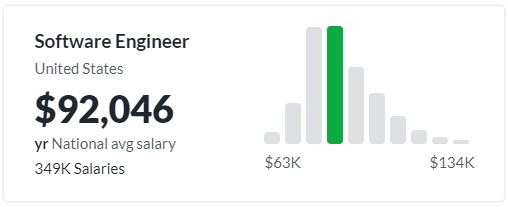
\includegraphics{glassdoor1}
\centering
\caption{Example of data and graph shown on glassdoor}
\label{fig: glassdoor-data}
\end{figure}

\noindent \textbf{Features:}
\begin{itemize}
\item anonymously collects company reviews and salary information (including job title, locations of position, years of experience, etc.)
\item job postings
\item company profiles with generic info (number of employees, revenue, etc.)
\item collects interview questions
\item shows aggregate salary information for job titles (average salary for software engineer in a country, bar chart showing distribution of salaries)
\end{itemize}
\medskip

\noindent \textbf{Design Choices:}
\begin{itemize}
\item Must submit a salary to view salary information. Otherwise, salary collection form is not that prominent. The link to add salary can be found under "salary" tab but it's not highlighted in any way.
\item Users define their job title - sometimes there are lots of close titles but it's unclear if they are the same.
\end{itemize}
\medskip

\subsection{Comparing Alternative Solutions}
The following tables compare the different features available across alternative solutions.
\medskip

\noindent \textbf{Legend}

\noindent 
\includegraphics{comparison-legend}
\medskip

\begin{figure}[h]
\noindent 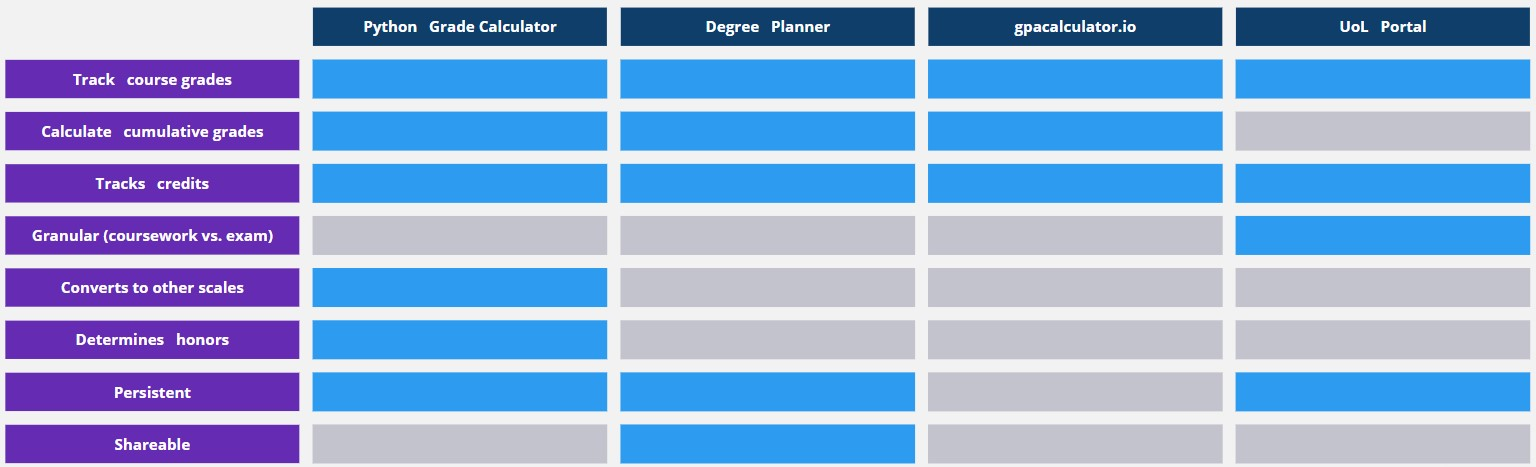
\includegraphics[width=\textwidth]{comparison-table-tracking}
\caption{Grade Tracking Comparison Table}
\label{fig: comparison-table1}
\end{figure}
\medskip

\begin{figure}[h]
\noindent 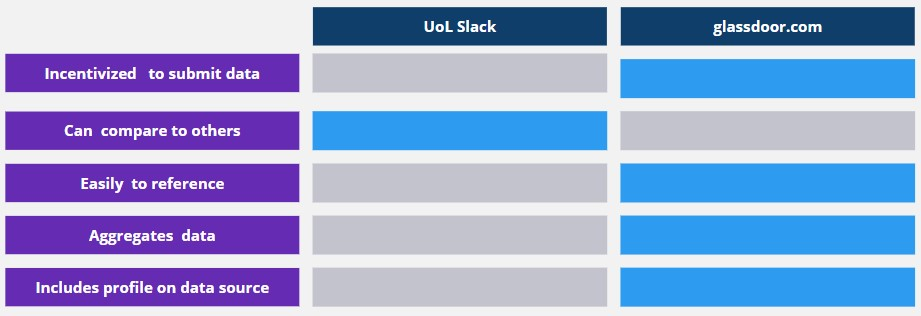
\includegraphics[width=\textwidth]{comparison-table-sharing}
\caption{Grade Sharing Comparison Table}
\label{fig: comparison-table2}
\end{figure}

\subsection{Our Solution's Place in the Market}
\textbf{SWOT Analysis}
\subsubsection{Strengths}
\begin{itemize}
    \item Knowing you have a relatively high grade could be motivating / encouraging / validating
    \item Validation if your grade was low but many people report similar grades
    \item Highlighting of potentially more challenging courses for future cohorts to allocate more focus and preparation on
    \item Highlighting when many people consider their grades unjustifiably low which may help in organizing a more detailed, thoughtful request to the institution to review the grades or rubric
    \item Motivation to maintain ones standing at or above a certain percentile
    \item Leaderboard aspect "gameifies" grades and gives incentive to submit grades
\end{itemize}
\subsubsection{Weaknesses}
\begin{itemize}
    \item Data reliability. We have no good way to validate data. We must disincentivize dishonesty and not assume 100\% accuracy.
    \item A small sample size of participants will limit usefulness of averages
    \item Those with poor marks or marks they feel are unjustified will likely be less willing to share
    \item Those who fail or drop out may be unable (depending on integration) or unwilling to participate, which will artificially inflate all grade averages
    \item Without a   representative sample of students, the averaged data, graphs, etc will be skewed and could lead to reduced acceptance or usage of the tool
    \item If we report anonymously, do we also store anonymously? If so then do we provide for the ability to remove data on request?
    \item If the tool is not completely opt-in / crowd-sourced then someone needs to moderate the data insertions and deletions.
\end{itemize}
\subsubsection{Opportunities}
\begin{itemize}
    \item This project has few real competitors. There are some student created utilities but grade sharing/comparing is outside the scope of those utilities.
    \item The program size will continue to grow for a long time. We haven't reached the maximum number of cohorts and the recent cohorts have grown. The need exists, there just wasn't a reason to make it until now.
    \item If we are the first to make this, we can capture the interested user-base which should be a large moat.
    \item Develop this as with Slack integration so it can naturally link to the community of students that already exists, leveraging the University's policing of that population to being actual students
    \item Add some flags for people to rank their grades. Perhaps they felt the grade was unjustified, or that it was boosted or dragged down by group participants or life events (ie, only receiving a 50\% in a course while feeling stress from COVID)
    \item Provide a field for students to provide short advice to others for each course they provide a grade for
    \item Store the user's grades for visibility of all their courses at once, which if public could be summarized quickly for sharing to others
    \item Provide an overall average per course, per semester, etc to help future students know what to expect and perhaps how much they need to prepare
    \item Provide for grade conversions using various methodologies to non-UK standards
\end{itemize}
\subsubsection{Threats}
\begin{itemize}
    \item Time. Other student utilities show recognition of value for this type of product. Probably only a matter of time until someone else extends the grade idea in a similar fashion.
    \item Leak or theft of personally identifiable grade and contact information
    \item People could poison the data with dishonest grade reporting
    \item If the tool is completely opt-in / crowd-sourced ...
    \begin{itemize}
        \item ... and we allow the removal of information then perhaps people would remove other people's data
    \end{itemize}
    \begin{itemize}
        \item ... people may impersonate other people along with reporting their real or falsified grades
    \end{itemize}
    \item Loss of integrations / changes to any APIs we're using
    \item Data loss - backups
\end{itemize}
\section{Planning and Requirements Gathering}
\subsection{Methodology}
\textit{You should focus on how you hope to plan and gather requirements. We discussed some different methods in the lectures and discussion group activities. It is important that you evaluate the different methods in making your decisions and provide some written analysis in your reports, with clear critique and some functional understanding for the higher marks.}
\subsection{High-Level Requirements Funnel}

\subsection{Implementation Approach}

\section{Formative Testing and Evaluation}
\subsection{Identifying Users}
\textit{This is the part of the project which requires the most research and understanding. For middle marks, you should provide a good, clear overview of techniques to identify and sample users, with a set of contextually relevant information and a balanced overall argument. This should bridge cohesively with your requirements engineering techniques, as well as your general research in target demographics, types of systems and processes involved}
\subsection{Testing \& Evaluation Methods}
\textit{Higher marks would require rigorous tests that are insightful and utilise a wide range of metrics to analyse success through different lenses.}


\subsection{}

\section{Prototyping Techniques}
\textit{You should describe your prototype, where strengths in different techniques lie and where they are used. This section should also detail the movement between low- fidelity and high-fidelity techniques, with a view to building the system and the types of technology involved. There should be evidence of iterative design and evaluation steps.}
\subsection{Techniques}
\subsection{Low-Fidelity Prototypes}
\subsection{High-Fidelity Prototypes}

\section{Evaluation Techniques}
\subsection{Critical Success Factors}
\textit{Where do the critical success factors lie and what novel techniques could you use to measure your work?}

\subsection{Measurement of Success \& Failure}
\textit{How do you intend to measure success and failure in context? }

\subsection{Results}
\textit{ What works well about the system and where are the fundamental flaws?}


\end{document}
